\documentclass{article}
\usepackage{tikz}
\usetikzlibrary{shapes.arrows}%for the blue arrows
\usepackage{amsmath}%For array
\usepackage{caption}%For including figures or other not accepted environments in minipage
\usepackage{tcolorbox}%For the colorbox
\usepackage{lipsum}%for pseudo-random text


\begin{document}
\lipsum[1]
\vspace{\baselineskip}

\noindent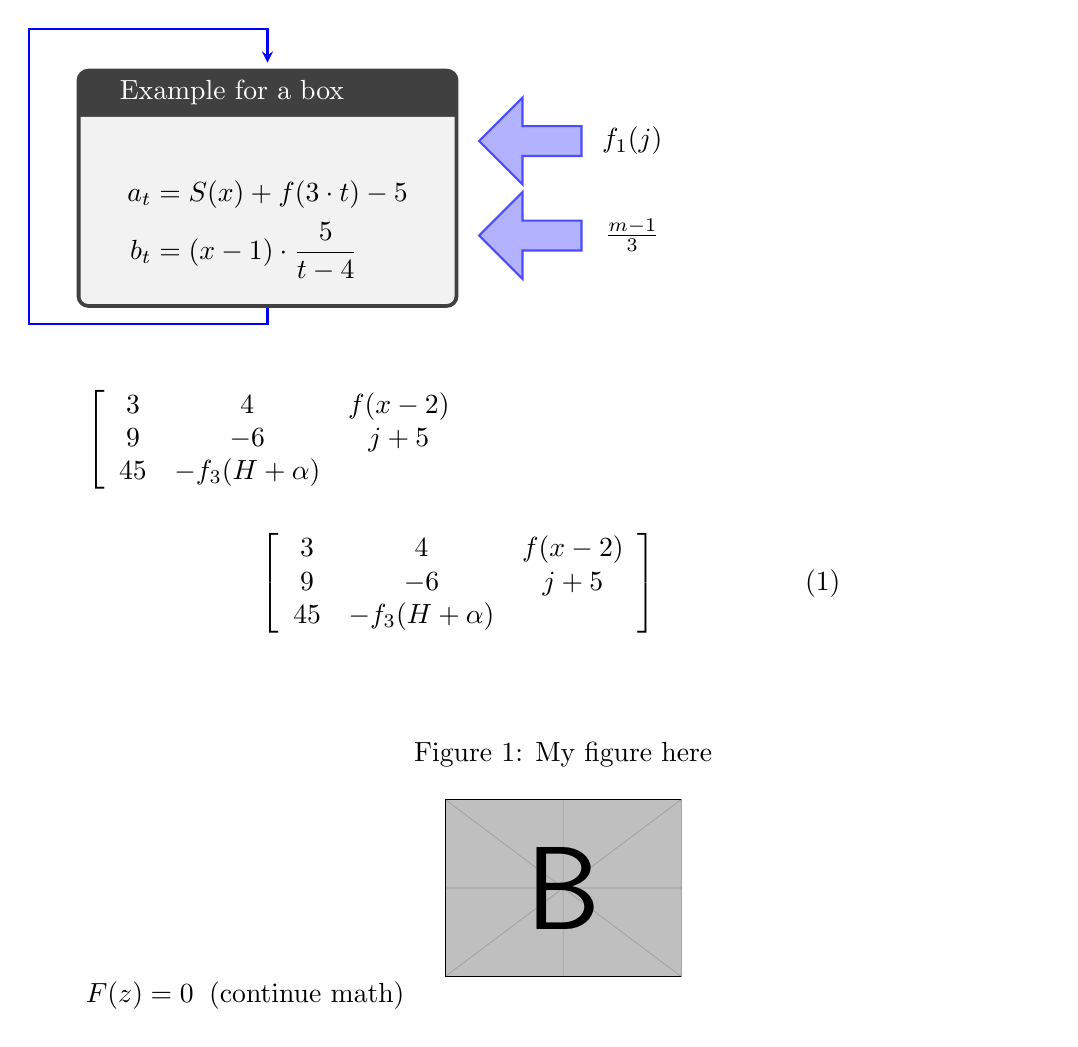
\begin{tikzpicture}
    %Arrow style from here : https://tex.stackexchange.com/a/247875/120578
    \tikzset{>=stealth,->,shorten >=2pt,looseness=.5,auto,shape border rotate=180,
    fat arrow/.style={single arrow,
                          thick,draw=blue!70,fill=blue!30,
                          minimum height=13mm,minimum width=11mm}}
  \coordinate(TopLeft);
  \node[anchor=west,inner sep=0](First) at(TopLeft)
       {\begin{tcolorbox}
           [width=0.4\textwidth,title={Example for a box}]
           \begin{align*}a_t&=S(x)+f(3\cdot t)-5\\
             b_t&=(x-1)\cdot\frac{5}{t-4}
           \end{align*}\end{tcolorbox}};
       \coordinate (mbot)at (First.south);
       \coordinate (mtop)at (First.north);
       \coordinate (mleft)at (First.west);
       \coordinate (mright) at(First.east);
       \draw[thick,blue,->] (mbot)|-([yshift=-0.2cm]mbot)-|([xshift=-0.6cm]mleft)|-([yshift=0.5cm]mtop)-|(mtop);
       \node (J)at ([xshift=1cm,yshift=0.6cm]mright)[fat arrow]{};
       \node at ([xshift=1.2cm]J){$f_1(j)$};
       \node (K)at ([xshift=1cm,yshift=-0.6cm]mright)[fat arrow]{};
       \node at ([xshift=1.2cm]K){$\frac{m-1}{3}$};
       \node[anchor=west] at ([yshift=-3cm]TopLeft) {\begin{minipage}{0.4\textwidth}\[\left[\begin{array}{ccc}3 &4 &f(x-2)\\
               9 &-6& j+5\\
               45 &-f_3(H+\alpha)
             \end{array}\right.\]\end{minipage}};
      \node[anchor=west,inner sep=0] at ([yshift=-5cm]TopLeft) {\begin{minipage}{0.8\textwidth}\begin{equation}\left[\begin{array}{ccc}3 &4 &f(x-2)\\
               9 &-6& j+5\\
               45 &-f_3(H+\alpha)
              \end{array}\right]\end{equation}\end{minipage}};
      \node[anchor=west] at ([yshift=-8.5cm]TopLeft) {\begin{minipage}{\textwidth}\begin{center}\captionof{figure}{My figure here}\includegraphics[width=3cm]{example-image-b}\end{center}\end{minipage}};
                  \node[anchor=west] at ([yshift=-10cm]TopLeft) {\begin{minipage}{0.3\textwidth}\[F(z)=0\;\;\text{(continue math)}\]\end{minipage}};
\end{tikzpicture}

\end{document}